\section{Architettura} \label{section:architettura}

Per lo sviluppo generale dell'applicazione, è stata seguita una architettura DApp\glo{}, (Fully) Decentralised Application.
Essa consiste in un frontend Web che effettua chiamate dirette ad una infrastruttura decentralizzata backend, nel 
nostro caso una gerarchia di smart contracts eseguiti su blockchain Fantom; 
questa struttura ricorda quindi una architettura client-server, senza un supporto intermedio per le operazioni.
\\
Il pattern architetturale\glo{} scelto dal gruppo per lo sviluppo del frontend è il Model-View-ViewModel\glo{}. Il
seguente pattern è tra i più diffusi nello sviluppo delle web application e permette di scrivere codice
facilmente mantenibile e riusabile; questo è possibile grazie al forte disaccoppiamento che sussiste tra
logica di presentazione e di business. Inoltre l'MVVM è risultato il più adatto per essere utilizzato con
React, libreria impiegata per lo sviluppo dell'UI e che renderizza le componenti in base al loro stato\glo{} interno.

\begin{figure}[H]
    \centering
    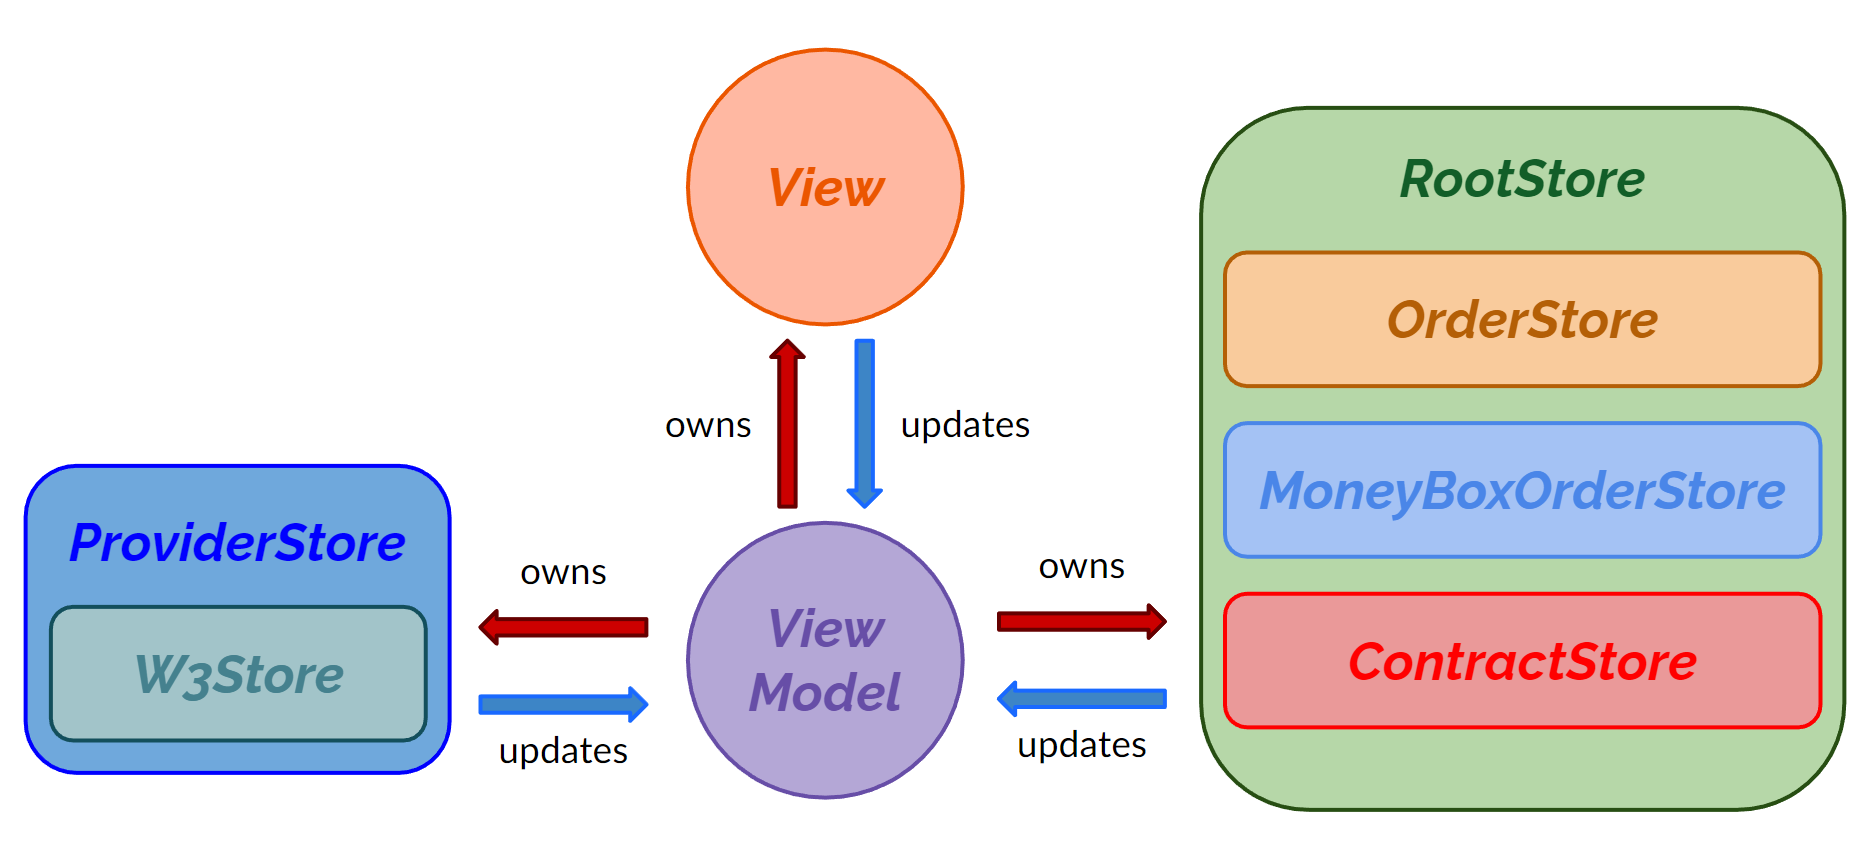
\includegraphics[scale=0.3]{immagini/mvvm.png}
    \caption{Model-View-ViewModel di ShopChain}
\end{figure}

Il passaggio dei dati dal Model alle varie componenti grafiche avviene attraverso l'utilizzo di un Context
React, al quale viene passato un'istanza del ViewModel. L'utilizzo di un Context React ci permette di
accedere al valore corrente del ViewModel in qualsiasi porzione della View, senza doverlo passare di
componente in componente attraverso le props (ossia gli argomenti dei componenti che compongono la
vista). Nella radice dell'applicazione viene infatti creata un'istanza del ViewModel, che viene passata
ad un Context.Provider, che fa da contenitore per tutta la View. All'interno di tale contenitore ogni
componente può utilizzare un hook per accedere al Context React ed utilizzare il valore più recente del ViewModel.
\\
È stato scelto di utilizzare un Context React per il passaggio dei dati in quanto la nostra applicazione è
molto profonda e non risultava conveniente passare i dati per molti componenti rischiando, nel peggiore
dei casi, di doverli utilizzare nell'ultimo della gerarchia.
Per poter fare in modo che una componente della View si renderizzi non solo al cambiamento del
suo stato interno ma anche al cambiamento dei dati nel Model, abbiamo utilizzato la libreria Mobx\glo{}.
Questa ci permette di implementare l'observer pattern\glo{}, non supportato di default da React. A tale
scopo, Mobx\glo{} permette di segnare delle classi (o attributi di esse) come observable\glo{} e di costruire
dei componenti della View come observer\glo{}. \\Quest'ultimi vengono automaticamente ri-renderizzati al
cambiamento di un qualsiasi attributo observable.

\subsection{Diagrammi delle classi}

\subsubsection{Classi Frontend}

\begin{figure}[H]
    \centering
    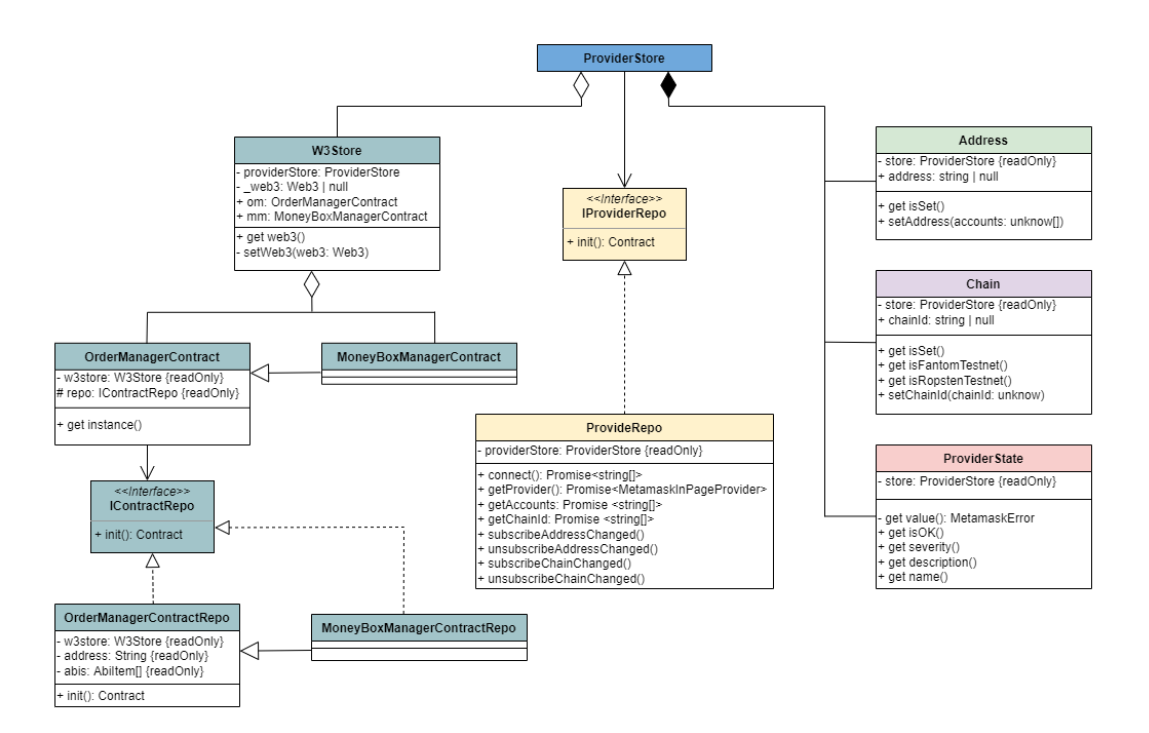
\includegraphics[scale = 0.5]{immagini/providerstore.png}
    \caption{La gerarchia di ProviderStore}
\end{figure}

Si può notare la struttura ad albero degli store, in questo caso particolare il Provider Store, 
il quale da come si può vedere fa ampio uso di ereditarietà proprio come avviene a livello di smart contract.
La classe singleton \textbf{ProviderStore} si occupa di gestire la connessione alla blockchain, tramite l'istanziazione di \textbf{W3Store}; 
l'istanziazione della connessione ai due contratti Order e Moneybox, 
l'istanziazione della  connessione ai due contratti per ordini e moneybox, l'address del wallet collegato \textbf{Address}, la tipologia di blockchain a cui si è collegati \textbf{Chain} e, con tutte le precedenti, 
ne deriva inoltre uno stato generale \textbf{ProviderState}, con relativi errori.
\clearpage

\begin{figure}[H]
    \centering
    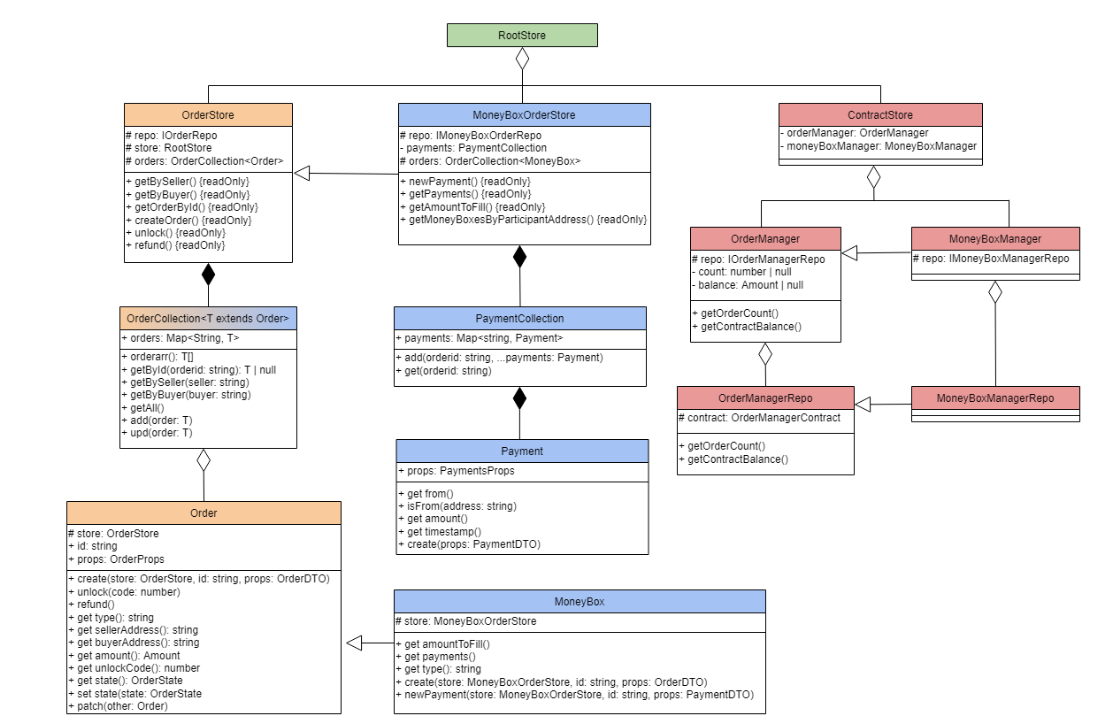
\includegraphics[scale = 0.5]{immagini/rootstore.png}
    \caption{Rootstore, le classi per gli ordini e la gestione dei contratti}
\end{figure}

Anch'esso con struttura ad albero, RootStore si occupa di gestire i dati di dominio, gli ordini singoli e moneybox e i pagamenti.
Ci sarà quindi \textbf{OrderStore} e classi relative che si occupa di gestire tutti gli ordini di base 
e \textbf{MoneyboxOrderStore} il quale estende OrderStore trattando non più ordini di base ma MoneyBox e aggiungendo la gestione dei pagamenti multipli.
Stessa cosa accade a livello di \textbf{ContractStore}, ma in maniera più semplice in quanto la differenza effettiva sta nella repository assegnata: in base al caso base (order) o al caso derivato (moneybox) il resto delle chiamate rimarranno invariate.

\begin{landscape}
\begin{figure}[H]
    \centering
    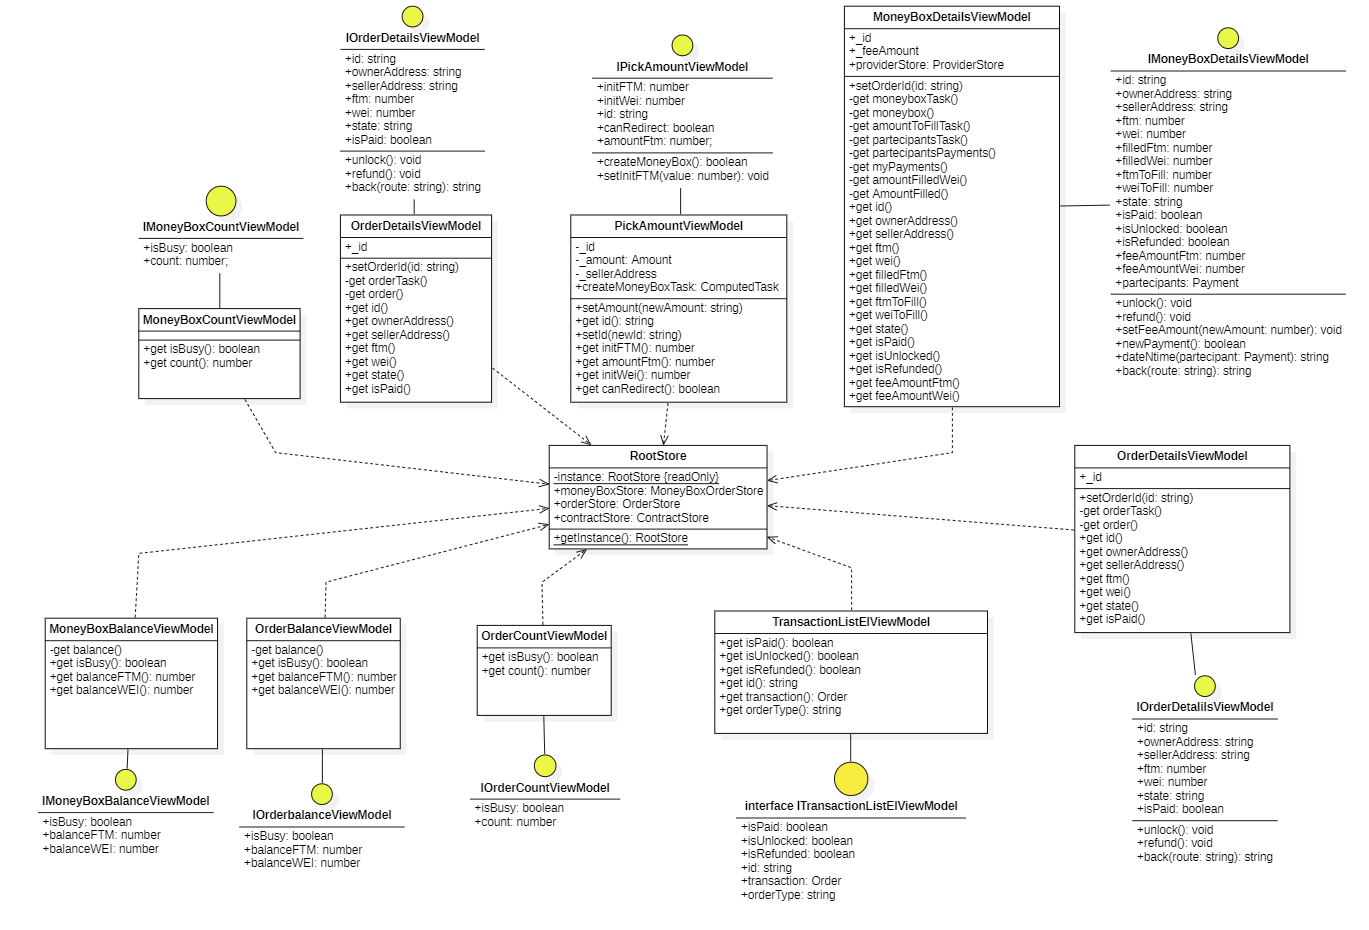
\includegraphics[scale = 0.6]{immagini/rsviewmodel.png}
    \caption{Le classi viewmodel dipendenti da RootStore}
\end{figure}
\end{landscape}

Da \textbf{RootStore}, dipendono poi la grande maggioranza delle classi ViewModel, ognuna con una sua interfaccia, che si occupano di gestire le chiamate dalla vista e apportare cambiamenti alla stessa.

\subsubsection{Classi Solidity}

\begin{figure}[H]
    \centering
    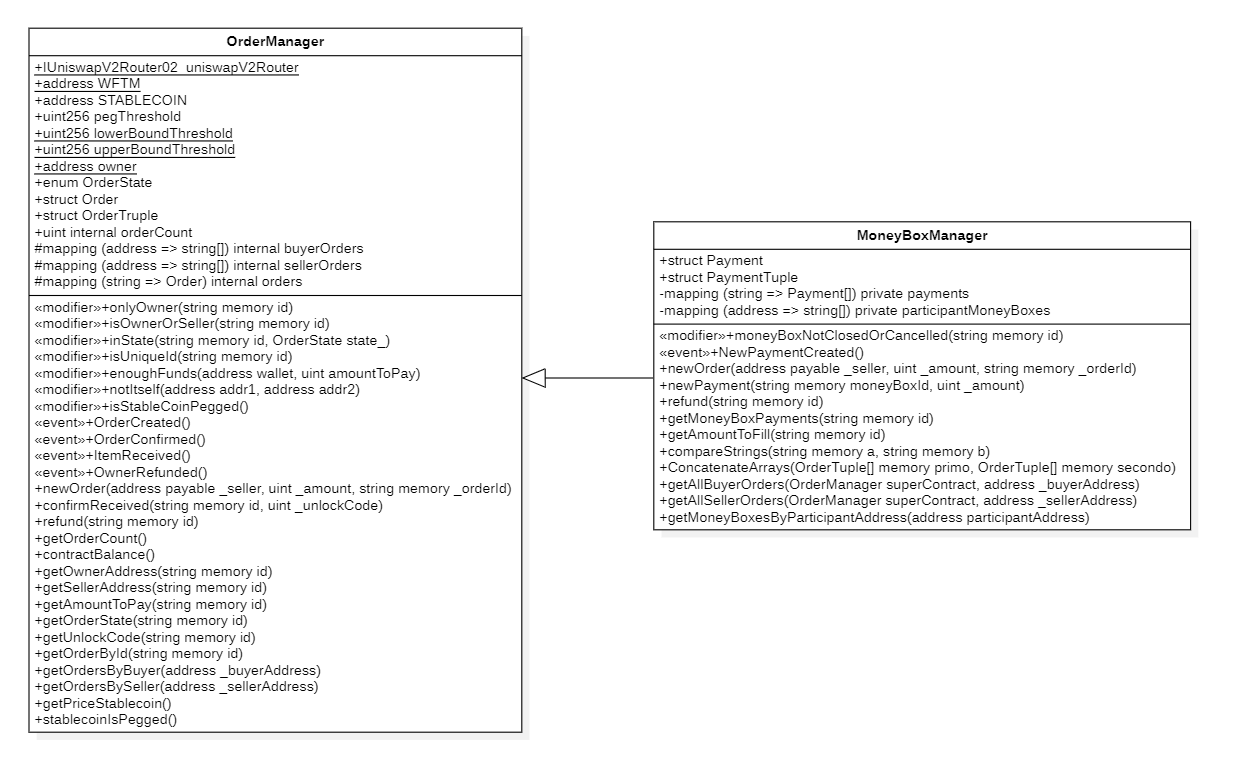
\includegraphics[scale = 0.5]{immagini/solidity.png}
    \caption{Le classi Solidity}
\end{figure}

Il diagramma delle classi Solidity, che gestiscono gli smart contracts, è stato creato seguendo le indicazioni di \href{https://github.com/naddison36/sol2uml}{\textbf{sol2uml}}.
Esso è costituito da due classi:
\begin{itemize}
    \item \textbf{OrderManager}, si occupa della gestione di tutti i pagamenti singoli, mappati per una migliore gestione degli stessi;
    \item \textbf{MoneyBoxManager}, si occupa della gestione delle Moneybox, anche esse mappate; essendo un'estensione di OrderManager, ne eredita tutti i metodi.
\end{itemize}

I primi sei attributi di \textbf{OrderManager}, e le funzioni \textit{isStableCoinPegged()}, \textit{getPriceStableCoin()} e \textit{stablecoinIsPegged()} 
servono alla conversione in stable coin\glo{} del pagamento effettuato in FTM, per garantire una maggiore stabilità della transazione. Per maggiori informazioni sulla implementazione della conversione in questo progetto, si visiti la sezione dedicata §\ref{section:conversione_stable}.\\
Tra i metodi, \textit{refund(string memory id)} si occupa di ritornare ai vari proprietari degli ordini 
(e a tutti i partecipanti nel caso di una MoneyBox) le somme di FTM interne al particolare contratto, identificato tramite \textit{id}.
\\
Per maggiori informazioni sulla parte generale dell'applicazione relativa alla Blockchain, si invita a consultare la sezione §\ref{section:blockchain}.



\subsection{Diagrammi di sequenza}

\begin{figure}[H]
    \centering
    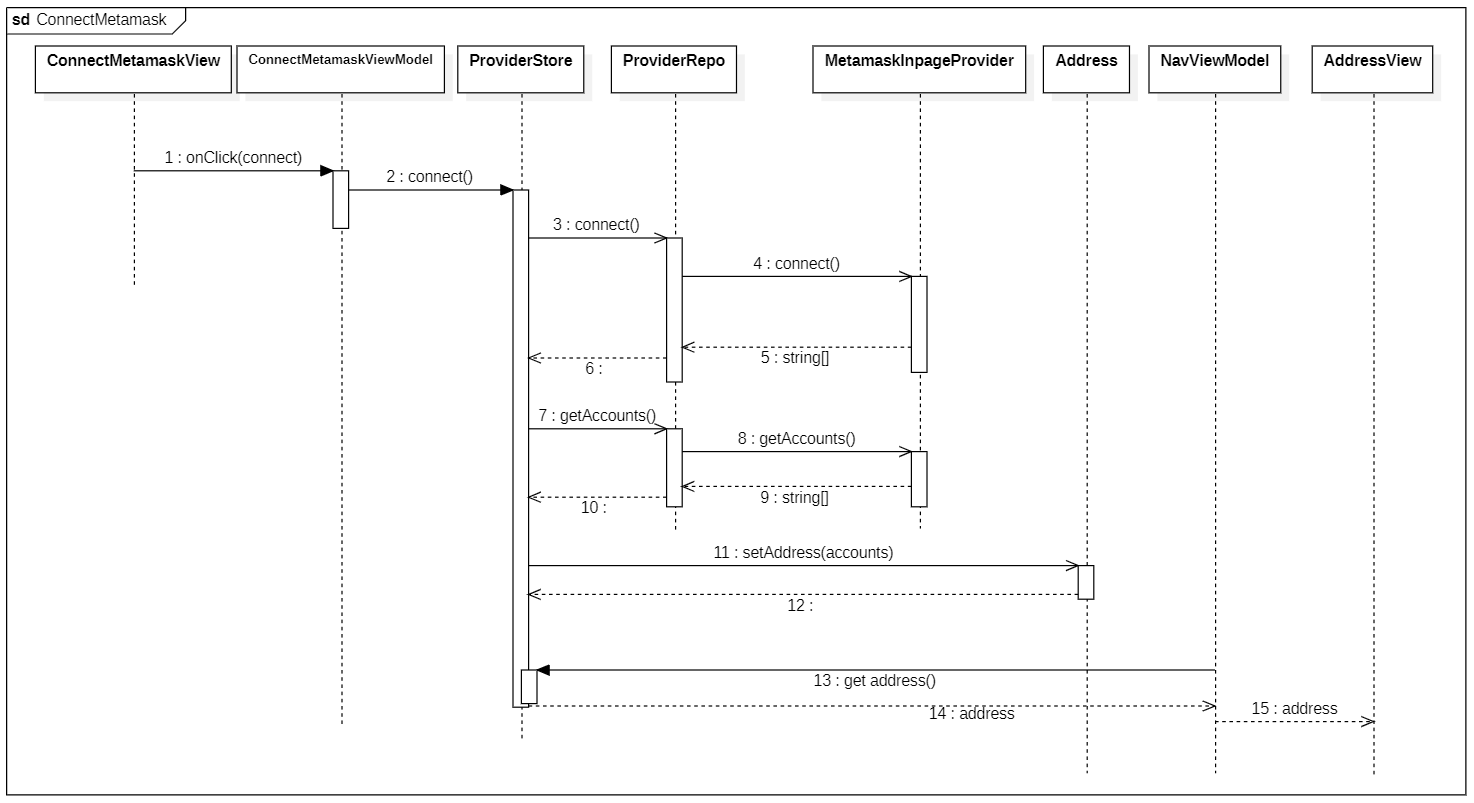
\includegraphics[scale = 0.45]{immagini/diagrammaMeta.png}
    \caption{Diagramma di sequenza per la connessione a Metamask}
\end{figure}

Il diagramma di sequenza sopra riportato è cosi descritto:

\begin{enumerate}
    \item La connessione a MetaMask inizia quando nella \textbf{ConnnectMetamaskView}, mediante l'apposito pulsante, viene fatto l'onclick e viene chiamato il metodo \textit{connect()} sul \textbf{ConnectMetamaskViewModel};
    \item Esso a sua volta chiama il metodo \textit{connect()} sul \textbf{ProviderStore} che a sua volta fa la chiamata asincrona del metodo \textit{connect} sul \textbf{ProviderRepo} che a sua volta fa la chiamata asincrona del metodo \textit{connect} su \textbf{MetamaskInpageProvider} e la connessione è così stabilita;
    \item Successivamente dato che potrebbero esserci più account connessi il \textbf{ProviderStore} chiama il metodo asincrono \textit{getAccounts} sul \textbf{ProviderRepo} che lo chiama a sua volta sul \textbf{MetaMaskInpageProvider}, il quale ritorna tutti gli indirizzi degli account connessi mediante un array di stringhe;
    \item Successivamente il \textbf{ProviderStore} setta l'indirizzo mediante il metodo \textit{setAddress} al quale viene passato in input il primo carattere dell'array di stringhe ritornato nel punto precedente;
    \item Infine la \textbf{NavViewModel} prende gli indirizzi connessi mediante il metodo \textit{getAddress} chiamato sul \textbf{ProviderStore}, e li ritorna alla \textbf{AddressView} per essere visualizzati.
\end{enumerate}

\begin{figure}[H]
    \centering
    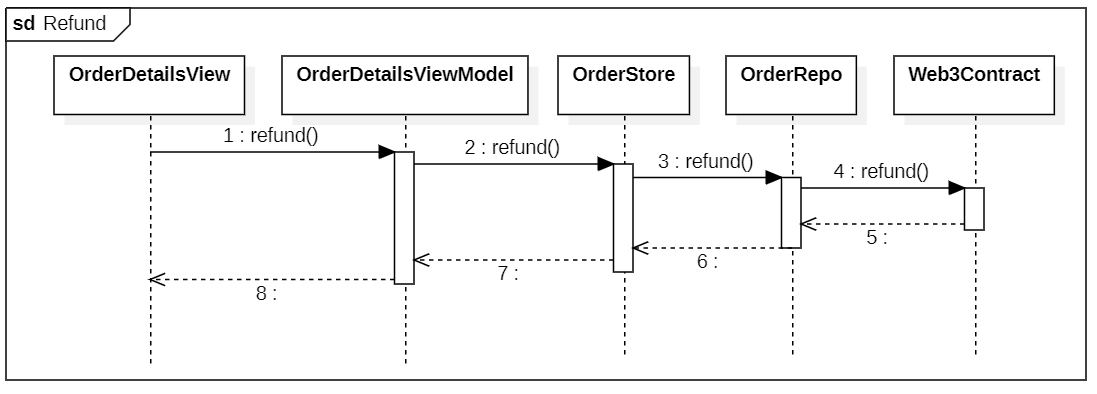
\includegraphics[scale = 0.6]{immagini/refund.png}
    \caption{Diagramma di sequenza della funzione di rimborso}
\end{figure}

Il diagramma di sequenza sopra riportato, molto semplice grazie ai pattern architetturali utilizzati, è cosi descritto:

\begin{enumerate}
    \item Dalla \textbf{OrderDetailsView}, dopo aver cliccato l'apposito bottone, parte la chiamata della funzione \textit{refund()} verso \textbf{OrderDetailsViewModel} per effettuare il rimborso dell'ordine corrente;
    \item Dal view-model, vengono chiamate le funzioni \textit{refund()} fino ad arrivare a Web3Contract, che si occuperà di contattare lo smart contract nella Blockchain;
    \item Al ritorno delle varie funzioni, l'utente visualizzerà un messaggio di avvenuto rimborso dei pagamenti.
\end{enumerate}

\clearpage
\subsection{Architettura di dettaglio}

\subsubsection{Repository pattern}

Il repository pattern è una astrazione del Data Access Layer (DAL\glo). Nasconde i dettagli su come esattamente i dati vengono salvati o recuperati dall'origine dati sottostante.\\
I dettagli sul modo in cui i dati vengono salvati e recuperati si trovano nel rispettivo repository.
Il repository pattern ci ha permesso di racchiudere tutte le interazioni il Data Access Layer (nel nostro caso la blockchain) in un oggetto unico, mantenendo la separazione tra implementazione e interfaccia. Tali Repository verranno utilizzati all'interno degli store, tramite Dependency Injection\glo{}.

\subsubsection{Singleton}

Sono state implementate alcune classi seguendo il design pattern Singleton,
 ciò consente di garantire che una classe abbia una sola istanza, fornendo al contempo un punto di accesso globale alla stessa.
Il design singleton è stato usato per avere un'unica fonte detentrice dello stato di ogni modello.
Le classi più importanti create seguendo il pattern singleton sono:

\begin{itemize}
    \item \textbf{RootStore}: classe che gestisce i dati di dominio, gli ordini, le moneybox e i pagamenti;
    \item \textbf{ProviderStore}: classe che gestisce la connessione a blockchain e tutte le classi relative, e l'istanziazione di W3Store;
    \item \textbf{W3Store}: classe che gestisce la connessione a Metamask.
\end{itemize}

\subsubsection{Observer pattern}

Attraverso Mobx abbiamo usato l'observer pattern in quasi tutte le classi del frontend in modo tale che, alla modifica di una classe observable, i cambiamenti si rifletteranno nelle classi observer.